\documentclass[11pt,a4paper,oldfontcommands]{memoir}
\usepackage[utf8]{inputenc}
\usepackage[T1]{fontenc}
\usepackage{microtype}
\usepackage[dvips]{graphicx}
\usepackage{xcolor}
\usepackage{times}
\usepackage[francais]{babel}

\usepackage[
breaklinks=true,colorlinks=true,
linkcolor=blue,urlcolor=blue,citecolor=blue, PDF VIEW
linkcolor=black,urlcolor=black,citecolor=black]{hyperref}

\usepackage{geometry}
% PDF VIEW
\geometry{total={210mm,297mm},
left=25mm,right=25mm,%
bindingoffset=0mm, top=25mm,bottom=25mm}
% PRINT
%\geometry{total={210mm,297mm},
%left=20mm,right=20mm,
%bindingoffset=10mm, top=25mm,bottom=25mm}

\OnehalfSpacing
%\linespread{1.3}

%%% CHAPTER'S STYLE
%\chapterstyle{bianchi}
%\chapterstyle{ger}
\chapterstyle{madsen}
%\chapterstyle{ell}
%%% STYLE OF SECTIONS, SUBSECTIONS, AND SUBSUBSECTIONS
\setsecheadstyle{\Large\bfseries\sffamily\raggedright}
\setsubsecheadstyle{\large\bfseries\sffamily\raggedright}
\setsubsubsecheadstyle{\bfseries\sffamily\raggedright}


%%% STYLE OF PAGES NUMBERING
%\pagestyle{companion}\nouppercaseheads 
%\pagestyle{headings}
%\pagestyle{Ruled}
\pagestyle{plain}
\makepagestyle{plain}
\makeevenfoot{plain}{\thepage}{}{}
\makeoddfoot{plain}{}{}{\thepage}
\makeevenhead{plain}{}{}{}
\makeoddhead{plain}{}{}{}


\maxsecnumdepth{subsection} % chapters, sections, and subsections are numbered
\maxtocdepth{subsection} % chapters, sections, and subsections are in the Table of Contents


%%%---%%%---%%%---%%%---%%%---%%%---%%%---%%%---%%%---%%%---%%%---%%%---%%%

\begin{document}

\thispagestyle{empty}
{
\sffamily
\centering
\Large

~\vspace{\fill}
\begin{center}

\includegraphics[height=1cm]{upmc.png}
\hspace{2cm}

\includegraphics[height=1cm]{lesfurets.png}
\end{center}
{\huge 
Modélisation des champs des champs des formulaires de LesFurets.com
}

\vspace{2.5cm}

{\LARGE
FITOUSSI Jonathan
}

\vspace{3.5cm}

Projet de fin d'études\\[1em]
Université Pierre et Marie Curie

\vspace{3.5cm}

Encadrant Université : CHAILLOUX Emmanuel\\
Encadrant Entreprise : DEGERBAIX Benjamin

\vspace{\fill}
\begin{center}
Aout 2015
\end{center}
}


\cleardoublepage
\tableofcontents*

\chapter{LesFurets.com}

\section{L'Assurance}
Le secteur de l’assurance fait partie du secteur économique tertiaire qui regroupe les
industries de services essentiellement immatériel. Il s’agit d’un secteur d’activité où les
acteurs économiques vendent une protection contre le risque avec un poids très important
au sein du paysage économique mondial et, plus particulièrement, au sein du paysage
économique français. Sa particularité réside dans son activité et sa diversité,puisque il
rassemble une multitude d’acteurs : compagnies d’assurance, courtiers, mutuelles, acteurs
internet, etc. Mondialement, le marché de l’assurance est actuellement dominé par les
états-Unis suivi par le Japon. La France occupe la 4ème position, derrière le Royaume Uni,
avec 6,5\% des cotisations mondiales, soit près de 211 235 millions d’euros. (FFSA
et Gema)

\section{Les comparateurs d'Assurance}
Un comparateur de prime d’assurance est un outil informatique permettant de comparer
toutes les offres d’assurances répondant à un ensemble de critères mentionnés par
le client. Avec un marché fortement concurrentiel et très complexe, les comparateurs ont
un rôle de plus en plus important auprès des clients en matière de comparaison, de choix
et de souscription de produits d’assurance. Aujourd’hui, le marché est occupé par des
concurrents connus tels que LeLynx.fr, LesFurets.com, Assurland.com, Hyperassur, automotocompare.fr,
kelassur.com, etc. En effet, ces comparateurs présentent des environnements
ergonomiques permettant aux visiteurs d’effectuer un comparatif de contrats auto,
moto, multirisques habitation, emprunteur ou santé, et de sélectionner les offres les mieux
adaptées à leurs attentes. Pour répondre aux besoins des clients, chaque acteur maintient son propre modèle qui repose sur plusieurs aspects : le tarif, la qualité des services proposés,
les services après-vente, les garanties, les franchises, les prestations, etc. Ainsi, chaque
comparateur présente des offres d’assureurs différents. Le référencement web et la publicité
présentent des investissements lourds pour l’ensemble des concurrents qui cherchent
à obtenir une visibilité conséquente auprès de leur clients. Les nouveaux arrivants doivent
forcément investir massivement pour trouver une place parmi les acteurs historiques sur
ce marché.

\section{Historique de l'Entreprise}
Courtanet, fondée en 2005 par Jehan de Castet, est la société éditrice du site AssureMieux.com.
Avec ses sites www.assuremieux.com, www.creditmieux.com, et son logiciel
Bénéfit, la société est devenue rapidement l’un des plus importants fournisseurs
français de solutions de comparaison d’assurances. Plus de 1 500 courtiers indépendants
français étaient équipés de ses solutions. Depuis Novembre 2010, Courtanet est majoritairement
détenu par BGL Group créé en 1992, intermédiaire britannique d’assurances et
propriétaire également du leader de la comparaison d’assurances en Grande Bretagne via
www.comparethemarket.com, qui a emporté 35% du marché au Royaume-Uni. Le groupe
est aujourd’hui structuré autour de quatre «piliers» : Entreprises intermédiaires, Entreprises
pilotées par marque (LesFurets.com), comparethemarket.com et services juridiques.
En Avril 2012, la plateforme de comparaison Assuremieux change d’identité et dé-
voile une nouvelle marque baptisée www.LesFurets.com, le comparateur qui « simpli-
fie » l’assurance. LesFurets.com est un comparateur indépendant et impartial d’assurance
auto, moto, santé, habitation et crédit. Sa mission est d’aider les consommateurs
à trouver l’assurance la mieux adaptée à leurs besoins au meilleur tarif. La mission
du site est d’apporter plus de transparence et de simplicité dans l’assurance. Ainsi,
il permet de comparer facilement les tarifs, les garanties, les franchises et les services
de grands assureurs auto, santé,moto, habitation et crédit. Son objectif est d’aider à
trouver l’assurance la mieux adaptée aux besoins des clients au meilleur tarif. Dans
le but d’offrir un service de qualité, LesFurets.com s’associe avec les plus grands assureurs
du marché : Direct Assurance, Amaguiz, IdMacif, Eurofil, AllSecur, Aon Asurances,
AcommeAssure, SOS Malus, Assurpeople, L’olivier Assurances, 4assur, EuroAssurance,
ActiveAssurances, AssurOnline, assurbike, aloa Assurances, SwissLife, Alptis, etc.
\chapter{Sujet de stage}
D’un point de vue technique l’équipe de lesfurets.com a décider d’abstraire les champs du formulaire ainsi que les dépendances à l’aide d'un méta-model. A l’heure actuelle, l’application web est capable de transformer ce modèle de champs au format XMI pour pouvoir les exporter dans un logiciel de modélisation comme MagicDraw, Rational. Le stage débutera par un passage à d’autres format de modélisation (EMF, JSON) traiter à l'aide d'outils open-source qui permettront aux équipes de mieux visualiser le graphe des champs des formulaires ainsi que leurs dépendances. Il est prévu ensuite de superposer des analytics sur ces graphes. Il est aussi envisager de garder une trace des différences entre les versions de l’application pour visualiser les modifications et/ou les régressions en fonctions des développements. Enfin au même titre qu’un IDE classique, l’outil devrai pouvoir proposer des fonctions d’édition, de sauvegarde et de partage des données traitées.

\section{Technologie}
Dans le cadre du projet, il me faudra explorer plusieurs piste :
La première consistera à me familiariser avec un outils de modeling basé sur Eclipse : Sirius (https://eclipse.org/sirius/overview.html). Sirius est un projet Open Source de la Fondation Eclipse. Cette technologie permet de concevoir un atelier de modélisation graphique sur-mesure en s'appuyant sur les technologies Eclipse Modeling, en particulier EMF et GMF. L'atelier de modélisation créé est composé d'un ensemble d'éditeurs Eclipse (diagrammes, tables et arbres) qui permettent aux utilisateurs de créer, éditer et visualiser des modèles EMF. Le projet est une initiative française et la communauté autour du projet est très active. Je me mettrais en relations avec les créateurs du projet pour pouvoir aborder les questions que j’aurais tout au long de mon stage.
Il me faudra aussi explorer la piste de la création une application web en charge d’afficher la modélisation. Il existe de multiple librairies en JavaScript pour l’affichage des données sous la forme de graphe orienté. De plus le il s'agit d'un graphe orienté faiblement cyclique qu'on pourra traitées, coté serveur avec des algorithmes implémenté en Java, Scala, Python ou JavaScript. Enfin aujourd’hui le graphe est généré sur un fichier au format XMI mais on pourrai imaginer que l’outil introspecte les objets directement dans les binaires.

\section{Objectif}
Les utilisateurs de l’outil seront d’une part les architectes logiciel de la société, les développeurs mais aussi les business-analyste (concepteur fonctionnelle) qui pourront mieux cerner les impacts des modifications ainsi que les besoin des utilisateurs du site lesfurets.com. Ainsi il faudra imaginer une interface qui pourrait s'apparenter à des wireframes qui ne sera plus l’apanage des seuls ingénieurs.
Fonctionnalités futures
Une fois l’outil développé et adapté aux besoin des formulaires, les équipes souhaiterait aussi modéliser l’arbre de dépendances des pages du site entre elle et de les liée aux donnée SEO déjà présentent.

\chapter{Problématique}

\section{Contexte}
L'application du site LesFurets.com est construite sur une architecture JAVA SE packager a l’aide de l'outils de gestion et d'automatisation de production des projets logiciels Maven. Maven s’occupe de gerer les dépendances de code générer certaines classes ainsi que de compiler le projet. Chaque formulaire est représenté au seins du site par un tunnel, toute la logique est est gerer par GWT (Google Web Toolkit) qui s’occupe de générer du code javascript depuis du code java. L'intérêt du framework est de permettre aux développeur java de l’entreprise d’aborder leur code coté client et coté serveur avec la même approche. De plus GWT met l'accent sur des solutions efficaces et réutilisables aux problèmes rencontrés habituellement par le développement AJAX : difficulté du déboggage JavaScript, gestion des appels asynchrones, problèmes de compatibilité entre navigateurs, gestion de l'historique et des favoris, etc.
Au seins de l’application il existe déjà un projet pour générer des fichiers mdxml et csv représentant les champs du formulaire c’est dans cette partie du code que l’on développera l’outils de modélisation.
Pour la modélisation en elle même Il s'agira essentiellement d'identifier les entités logiques et les dépendances logiques entre ces entités. La modélisation des données est une représentation abstraite, dans le sens où les valeurs des données individuelles observées sont ignorées au profit de la structure, des relations, des noms et des formats des données pertinentes.
Pour simplifié la problématique, l’équipe de LesFurets.com a décider d’abstraire les champs du formulaire ainsi que les dépendances à l’aide d'un méta model. Un méta modèle décrit la structure des modèles et permet de raisonner sur les modèles comme sur les connaissances de premier niveau.

\section{Génération de code générer}
Une fois l'Enum Java crée pour un champ du formulaire, les labels et d'autres caractéristiques du champ sont crée à l'aide de différentes Classes qui sont code-générer à différents moment lors de la compilation Maven. La première problématique qui se présente est de bien comprendre à quel moment sont généré les toutes les classes liées à ces champs. Toutes ces informations seront nécessaires par la suite.

\section{API Reflection}
Pour recuperer les bonnes informations dans le JAR il me faut utiliser une Api d'intropection. Pour cela il me faut comprendre comment fonctionne la compilation de Java, comment fonctionne un classloader et à quel moment je peux interroger mon api de réflection. Ensuite il faudra traiter les données récoltées pour les repartir dans des fichiers plats.

\section{Fichier de données}
Il a aussi fallu stocker dans des fichiers les données des champs du formulaires pour pouvoir y accéder rapidement. Ces données n'étant qu'en lecture seul, il n'y avais pas nécessité de les stocker dans une base de donnée. Le format XML est le format le plus utilisé dans l'application et il est facile de transformer une format mdxml en format xml simple. La difficulté se trouvera dans la fabrications de fichier JSON.

\section{Interface}
La partie interface dépendra de l'outil utilisé.

\subsection{Eclipse Sirius}
Dans le cadre de Eclipse Sirius, il faudra proposer une interface clair et un déploiement automatique sans qu'il n'y ai besoin de reprendre le système en main à chaque étape. Le placement des objet ainsi que leur design pourront se trouver dans la base de code et être interprèté comme le reste du projet pour détecter les erreurs. 

\subsection{Application Web}
Dans le cadre de l'application Web il s'agira de CSS et de JavaScript classique. Cependant il faudra placer l'application dans les pages de maintenances du site. Les pages de maintenance sont regrouper dans un package Java et il faudra rendre accessible les informations à ces pages ce qui n'est pour le moment pas le cas.

\subsection{Donnée Business}
Les données business sont disponible dans une base Olap dans laquelle on pourra lire sans risqué de perturbé le site. Plusieurs choix s'offre pour le traitement de ces données :

\begin{itemize}
\item Récupérer les données a l’instant ou la page est affiché 
\item Mettre en cache à des périodes données les données nécessaire
\item Réagir de manière réactive aux données mis a jour pour afficher une évolution des données en fonction des changement dans l’architecture des tunnels
\end{itemize}


\chapter{Analyse du problème}

Dans un premier temps ma démarche a ete de trouver une solution pour modéliser les champs du graph et de pouvoir les modéliser sous la même forme qu’il apparaisse sur le formulaire lui même. C’est a dire que l’idée etait d’observer le lien entre une champs texte “Avez vous déjà souscrit une assurance auto?” et une champs date “Quand avez vous obtenue votre permis de conduire”

\section{Eclipse Sirius}
Pour cela il m’a été suggérer d’utiliser un framework d’Eclipse : Sirius. Comme exposé plus haut Sirius est un outils spécialisé dans la modélisation de toute forme de problématique que peut se transposer en problème informatique.

\section{Application WEB}
Pour ma part j’ai aussi proposer une seconde solutiuon qui correspondait peut etre plsu a mon background. La solution etait d’utiliser  des library javasript pour visualiser les champs les layouter avec du HTML/CSS et de la propulser dans l’espace de maintenance de l’application en meme temps que le packaging de base

\section{Donnée Business}
Pour ma part j’ai aussi proposer une seconde solutiuon qui correspondait peut etre plsu a mon background. La solution etait d’utiliser  des library javasript pour visualiser les champs les layouter avec du HTML/CSS et de la propulser dans l’espace de maintenance de l’application en meme temps que le packaging de base

\begin{itemize}
\item Récupérer les données a l’instant ou la page est affiché 
\item Mettre en cache à des périodes données les données nécessaire
\item Réagir de manière réactive aux données mis a jour pour afficher une évolution des données en fonction des changement dans l’architecture des tunnels
\end{itemize}

\section{Autre utilisations}
Construire a l’aide de metamodel est une pratique courant chez lesfurets.com ainsi il m’est possible de réfléchir à d’autres utilisation de l’outils sans reprendre beaucoup la structure et le code utilisé. 

\subsection{Plan du site}
Les pages du site suivent une logique propre ainsi qu’un modele prédéfini avec comme information la JSP utilisé, la version mobile et la version desktop ainsi que les CSS utilisées il m’est ainsi possible de mettre en place un graph de toutes les pages avec les données sus-mentionnée. De plus si les liens proposé dans le site qui sont aujourd’hui des strings était remplacer par des valeurs dans le code on pourrait en plus visualiser le mail complet du site sans parcourir tout le code de chaque page a la recherche d’attribut href.

\subsection{CRM - Envoi de mail}
Lesfurets.com disposent d’un outils leur permettant d’envoyer des mails de services a leur client. Tous les champs utlisé dans ces mails sont present dans le codes et on pourrai proposer dans l’outil un moyen de visualisé les mails et leur dependances vers les champs existant
\chapter{Solution}

\section{Eclipse : Sirius}
Les premiers début du développement d’un modele pour Eclipse Sirius fut très fastidieux, après avoir passé un bout de temps sur le tutorial présent sur le site je me suis confronté a un manque d’autres exemples me permettant de vraiment prendre en main Sirius. Le manque d'information à été combler par l'équipe en charge du développement de Sirius. Cependant les démarches pour disposer d'une formation dans leur locaux à Nantes a pris trop de temps pour differentes raisons et nous avons du mettre de coté cette partie de la solution.

\section{Application Web}
Ma premier démarche a été de trouver une bibliothèque Javascript capable de generer un graphe orienté cyclique. Google m’a diriger vers une question similaire sur stackoverflow. J’ai bénéficier d'un comparatif complet des existent sur le net, avec leur avantages et inconvénient. Mon choix s’est porter sur cytoscape.js. Cytoscape avait l’avantage de réaliser rapidement un graphe correspondant à mes besoin depuis un fichier JSON. Il offre de plus une integration avec jQuery et/ou Angular pour la manipulation du DOM. Il est sous licence GPL ce qui faisait partie des impératifs du projet. Enfin Cytoscape propose par defaut une dizaine de layout utilisable pour explorer de différentes manière le graphe.
\clearpage
\section{Développement de l'outil}

\subsection{Tableau Json}
La première chose pour pouvoir exploiter un affichage du graphe des champs du formulaire avec Cytoscape est de générer un fichier Json. Le fichier contenant une liste d'objet représentant soit un noeud soit une arête. 
\begin{lstlisting}
elements: [
      { data: { id: 'foo' }, group: "nodes" },
      { data: { id: 'bar' }, group: "nodes" },
      { data: { id: 'baz', source: 'foo', target: 'bar' }, group: "edges" }
    ]
\end{lstlisting}
En se servant de la bibliothèque de Google Gson qui permet de transformer un objet Java en objet Javascript, il a été necessaire de créer des classes correspondant aux critères de Cytoscape. Il a fallu par la suite générer un fichier pour chaque tunnel au format Json contenant chaque champs avec les données qui lui sont propres et les dépendances sous formes d'arètes.

\subsection{Génération du graphe}
La logique par la suite était de servir les fichiers Json de façon asynchrone à la demande d'affichage du graphe d'un des tunnels de LesFurets.com. Pour cela la solution vers laquelle je me suis tourner était la manipulation du DOM à l'aide de AngularJS. Cytoscape permet à l'aide de closure de modifier le graph qu'en cas de modifications défini dans le "controller" AngularJS. 
\vspace{0.2in}
\begin{figure}[!ht]
\center

\includegraphics[width=15cm]{outil/buttons-tunnels.png}
\caption{Choix du tunnel}
\end{figure}
Ainsi à chaque demande du graphe d'un tunnel à l'aide d'un des bouttons de l'interface on demande si le tableau Json existe. Si il existe on trace le graphe sinon on fait un appel au serveur, une fois le fichier récu on lance le calcule du graphe. Si il y a une attente, on affichera un élégant loader invitant l'utilisateur à prendre son mal en patience.

\subsection{Zoomer, Déplacer les éléments, Se déplacer}
Une fois le graphe affichée il est apparu essentiel de pouvoir laisser l’utilisateur zoomer, se déplacer dans le graphe et déplacer les éléments du graphe. A l'aide de la documentation de l'API et aux fonctionnalités permises par la balise canvas de HTML5, j'ai pu définir des fonctions de glisser déposer pour déplacer les éléments ainsi que pour déplacer tout le graphe. Enfin pour les fonctions de zoom j'ai défini le graphe en position relative.
\clearpage
\subsection{Layout du graphe}
Cytoscape dispose d'un système pour permettre aux développeur de définir leur layout. Un layout n'étant qu'un ensemble de règles défini pour afficher les noeuds et arêtes sous forme de graphe.
\begin{lstlisting}[caption=Exemple d'un layout traçant le graphe sous forme de cercle]
var layoutCircle = {
  name: 'circle',
  fit: true, // whether to fit the viewport to the graph
  padding: 30, // the padding on fit
  boundingBox: undefined, // constrain layout bounds; { x1, y1, x2, y2 } or { x1, y1, w, h }
  avoidOverlap: true, // prevents node overlap, may overflow boundingBox and radius if not enough space
  radius: undefined, // the radius of the circle
  startAngle: 3/2 * Math.PI, // the position of the first node
  counterclockwise: false, // whether the layout should go counterclockwise (true) or clockwise (false)
  sort: undefined, // a sorting function to order the nodes; e.g. function(a, b){ return a.data('weight') - b.data('weight') }
  animate: false, // whether to transition the node positions
  animationDuration: 500, // duration of animation in ms if enabled
  ready: undefined, // callback on layoutready
  stop: undefined // callback on layoutstop
};
\end{lstlisting}
Enfin on laissera la possibilité à l'utilisateur de choisir le layout dont il aura besoin.
\begin{figure}[!h]
\centering
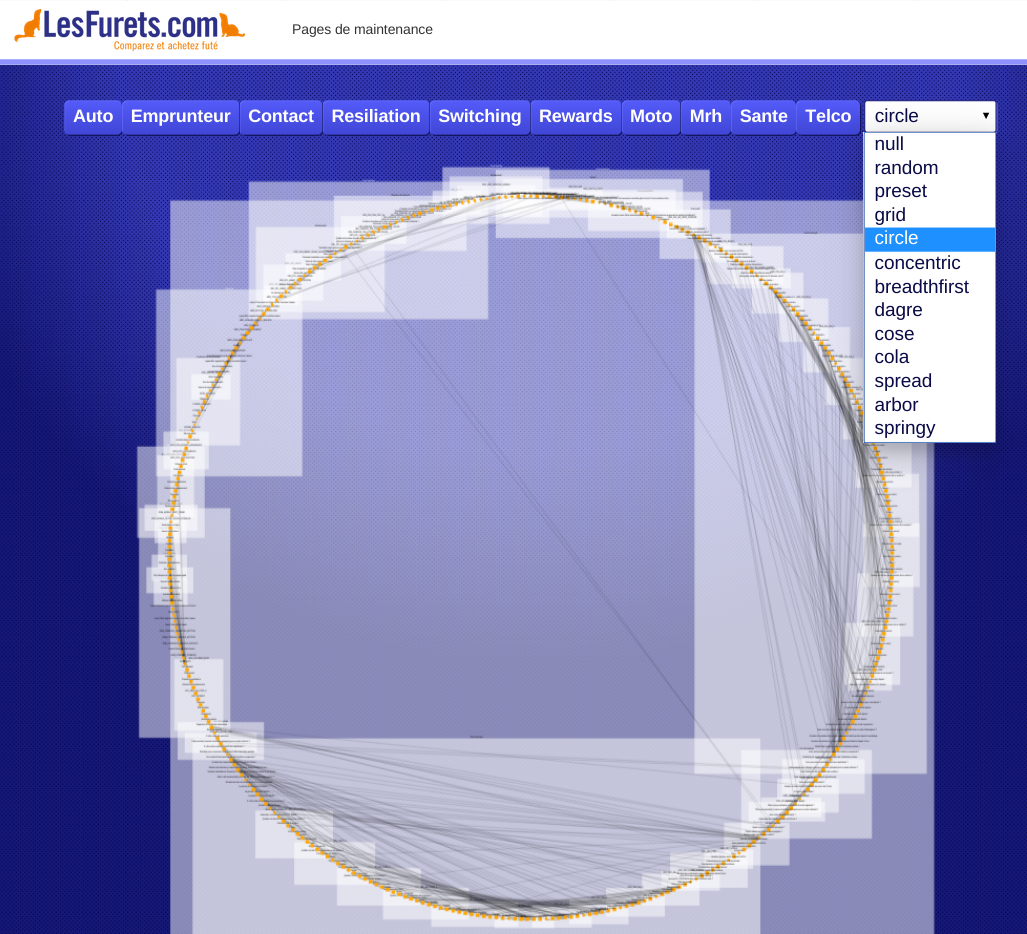
\includegraphics[height=10cm]{outil/layout-circle.png}
\caption{Graphe tracé avec un layout "circle"}
\end{figure}

\subsection{Layout WireFrame}
On proposera un layout "wireframe" qui permettra d'afficher le graphe sous une forme similaire au formulaire proposé dans les tunnels du site. C'est a dire que tous les écrans sont disposer à la suite les uns des autres et que sont disposé à l'intérieur, verticalement, les champs du formulaire. 
Pour cela il m'a fallut réaliser deux opérations non triviales : 
\begin{itemize}
\item 
Modifier la structure du Json pour inclure une donnée permettant de définir l'ordre des des écrans, blocs, groupes, champs du formulaire.
\item
Écrire une fonction dans mon Javascript permettant de positionner horizontalement et verticalement les éléments.
\end{itemize}
\vspace{0.5in}
\begin{figure}[!h]
\centering
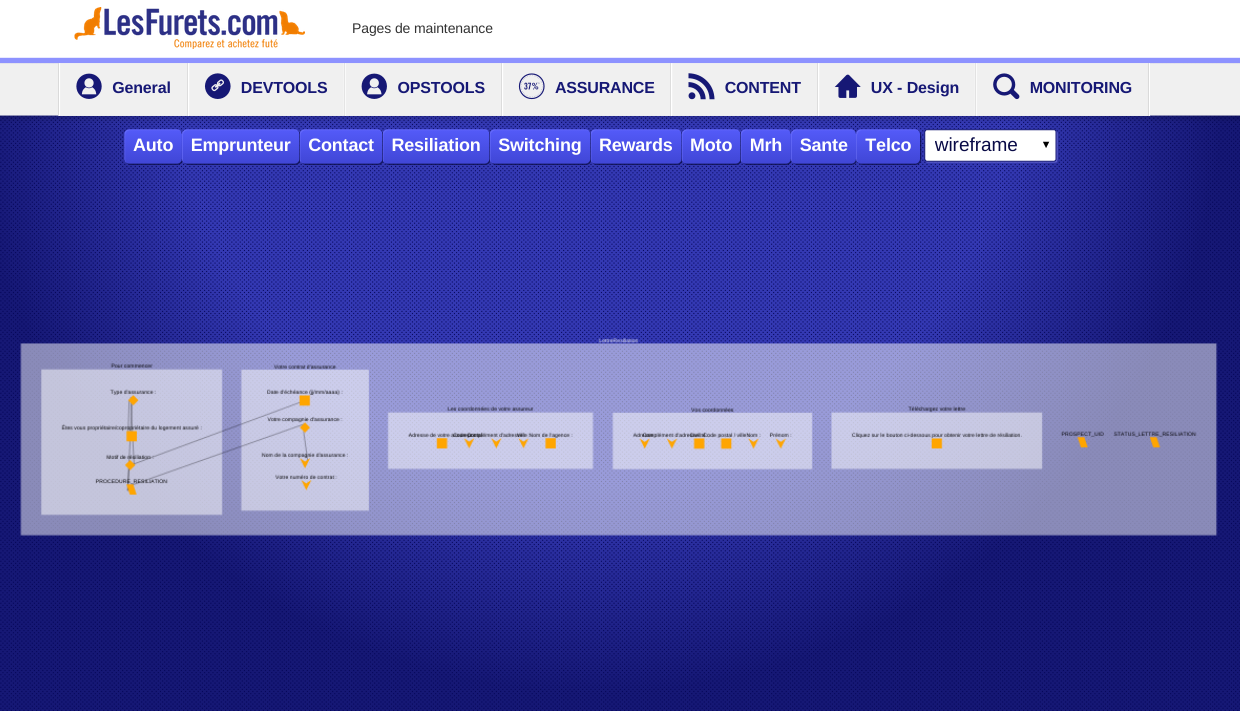
\includegraphics[width=15cm]{outil/layout-wireframe.png}
\caption{Tunnel Résiliation avec le Layout Wireframe}
\end{figure}

\clearpage
\subsection{Layout DAG}
On proposera aussi un layout "dag" qui affichera le graphe avec en évidence les cycles et les dépendances plus fortes. Pour cela on calculera les dépendances entres les champs. On calculera le score de chaque élément en fonction de son nombre d'arête total liée a un élément parent diffèrent, que ce soit un écran, un bloc ou un group. Enfin on disposera au plus proche les éléments contenu en fonction des deux éléments contenu ayant les plus grands score. Ce layout sera intéressant pour des tunnels avec un grand nombre d'élément pour visualiser les dépendances entres les éléments du formulaire.
\vspace{0.5in}
\begin{figure}[!h]
\centering
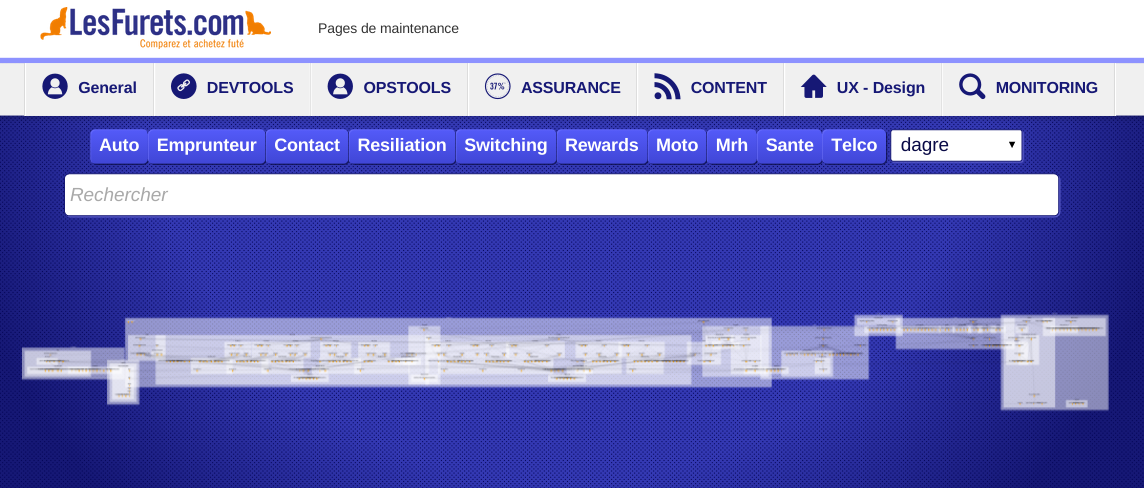
\includegraphics[width=15cm]{outil/layout-dagre.png}
\caption{Tunnel Assurance Auto avec le Layout DAG}
\end{figure}

\subsection{Recherche d’un champs et autocompletion}
Une fois la graph affichant tous les champs du formulaire il nous a paru nécessaire de pouvoir rechercher un champs et de pouvoir zoomer sur celui-ci. Ma première approche était d'écrire une fonction capable de zoomer sur un élément du graphe depuis le code. Une fois celle-ci implémenter, il à été facile de zoomer sur le champs et par la suite de zoomer sur son élément parent direct.
\vspace{0.5in}
\begin{figure}[!h]
\centering
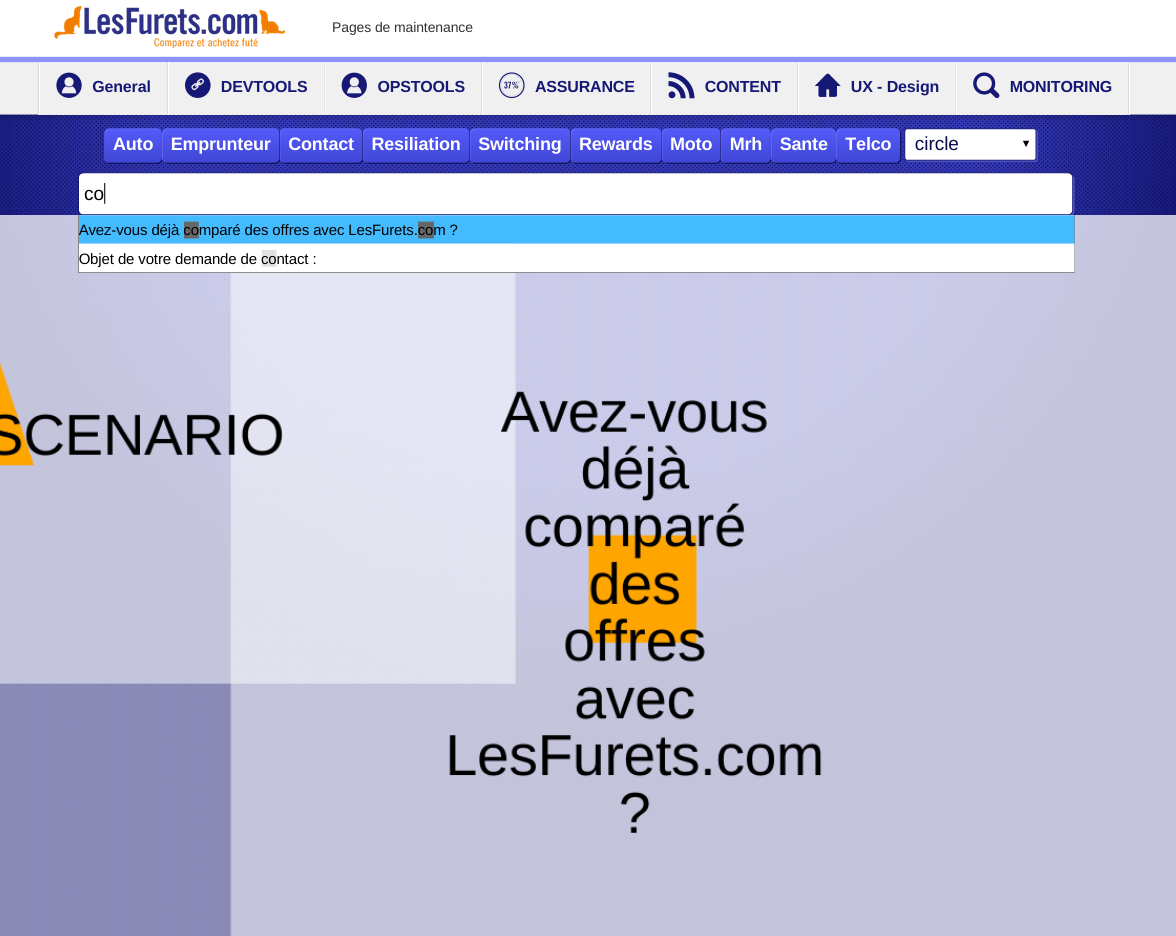
\includegraphics[height=5cm]{outil/feature-search.png}
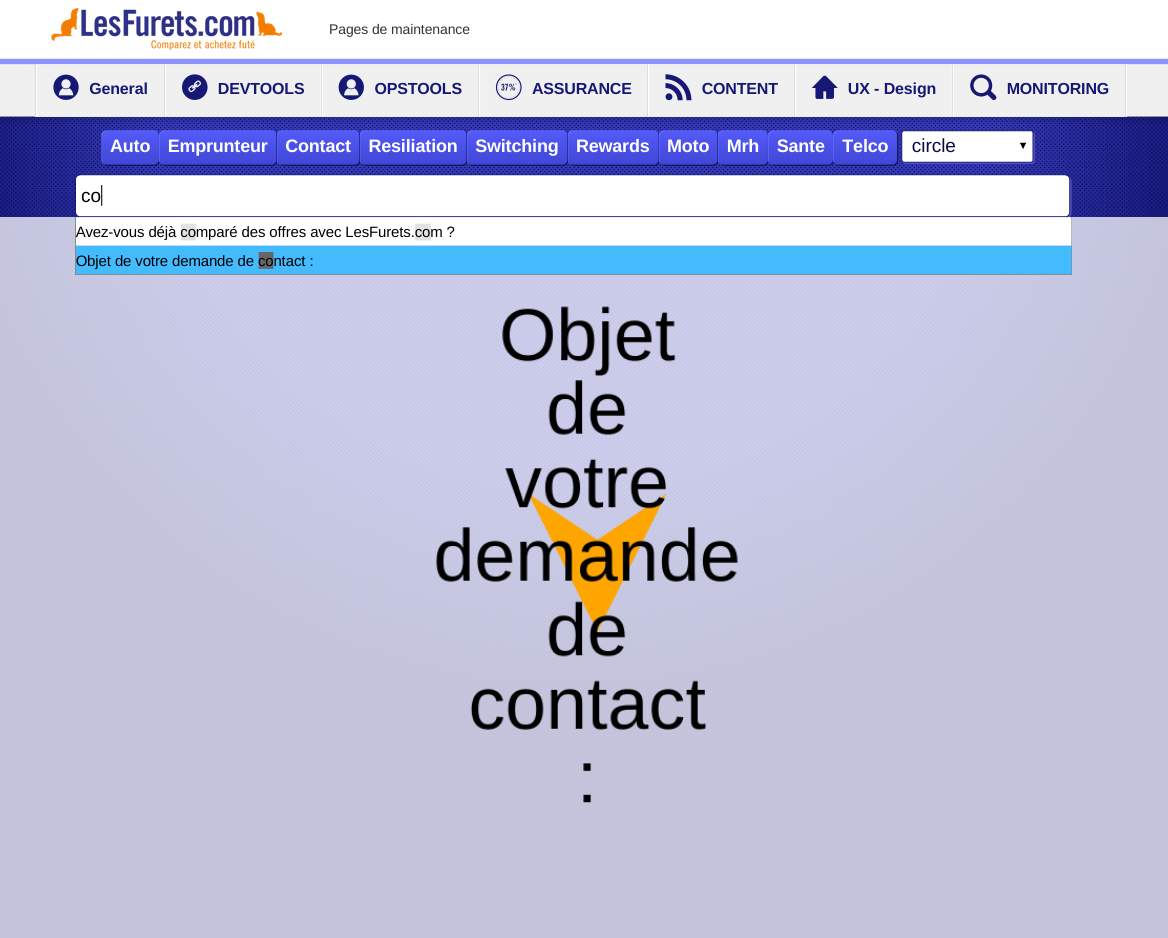
\includegraphics[height=5cm]{outil/feature-search-2.png}
\end{figure}

\subsection{Champs du formulaire}
Un autre gros morceaux du problème était de pouvoir afficher chaque champs d'après un style semblable a celui présent dans les champs du formulaire. Après avoir récupère une liste de tous les types d'éléments dans le formulaire : bouton, textbox, checkbox, boutons radio, liste, date, ... Cette liste était disponible depuis une Enum Java. Ensuite il a fallu dessiner dans la balise canvas des éléments ayant la forme des champs du formulaire.

\vspace{0.5in}
\begin{figure}[!h]
\centering
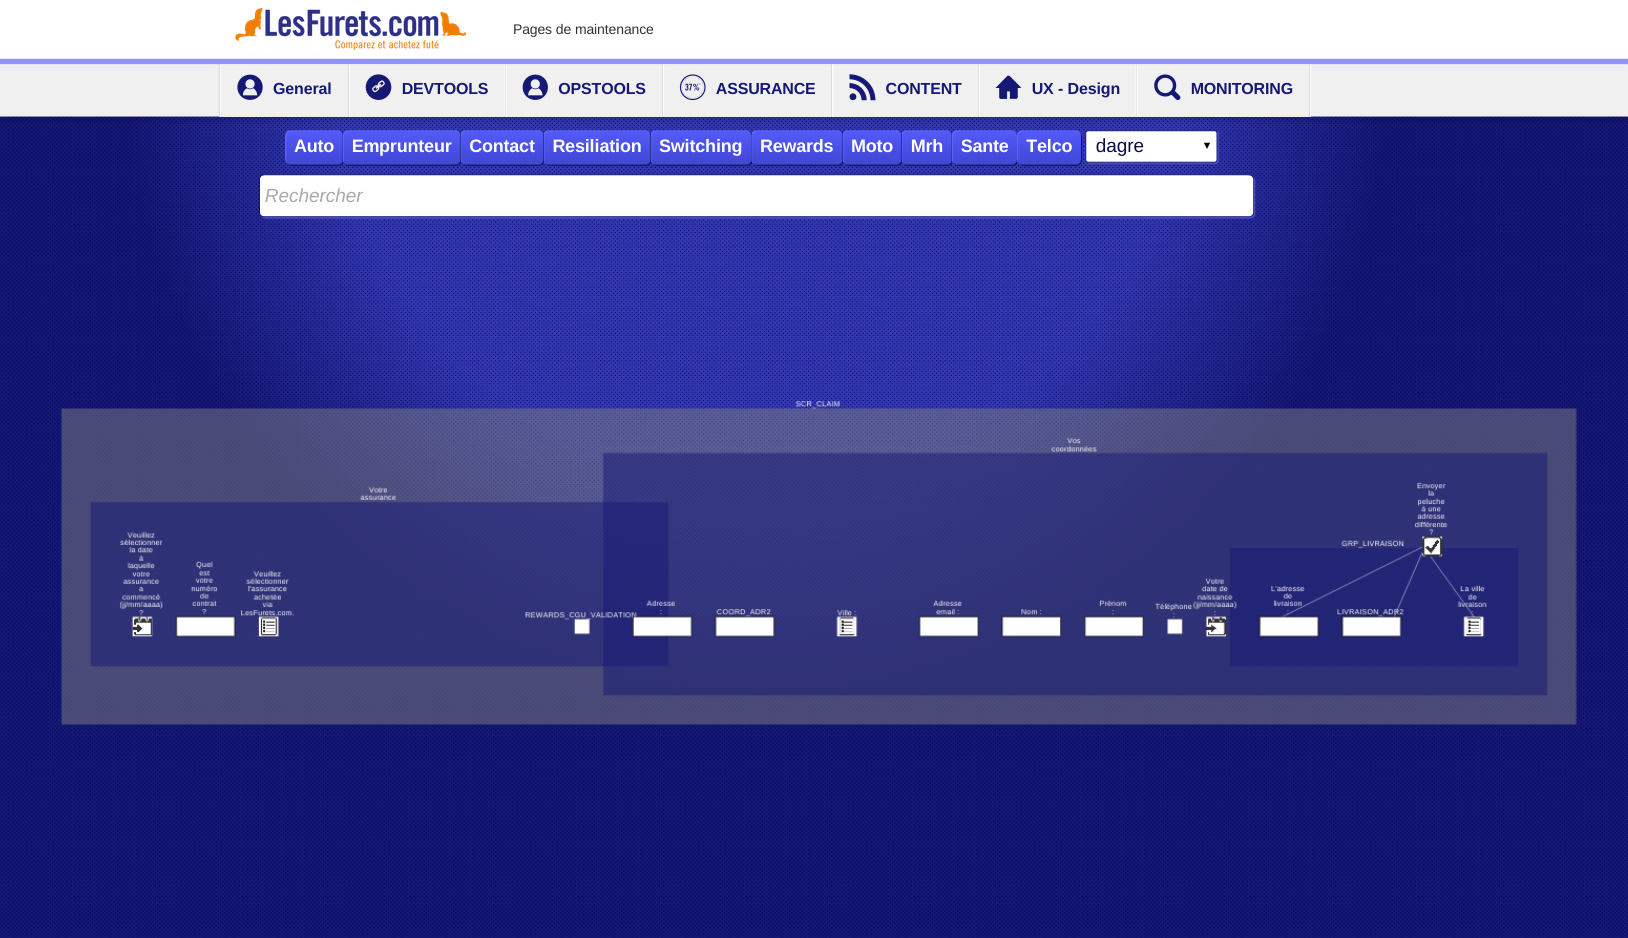
\includegraphics[height=9cm]{outil/layout-fields-2.png}
\caption{Différents type de champs du formulaire}
\end{figure}


\subsection{Modification des éléments et des dépendances}
Une fois la phase de "Layout" réalisé il a fallu mettre en place des fonctions de modifications/suppression des éléments du graphe. Et une fonction de modifications des dépendances entre les champs.

\subsubsection{Modification du label du champs}
La première fonction était sans doute celle qui avait le moins d’incidence sur le formulaire. Il s'agit de proposer aux utilisateur de pouvoir changer le nom du champs du formulaire.

\subsubsection{Modification type du champs}
On proposera aussi à l'utilisateur de pouvoir changer le type d'un champ sélectionné. Pour cela il a fallu lister tous les types de champs disponible. J'ai pu servir directement dans la JSP la liste des types de champs possible à l'aide d'une Enum présente dans le code Java.

\subsubsection{Suppression d’une dépendance}
Il s’agit juste de mettre en évidence les champs touché par la suppression d’une dépendances. Les dépendances ne sont pas interdépendantes. On soulignera les champs impacté par la suppression d'une couleur rouge.

\subsection{Sauvegarde du graphe}
Une fois les fonctions de modifications mise en place il a paru évident qu’il a fallait pouvoir sauvegarder l’etat du graph modifié pour pouvoir l’envoyer par la suite.
La premiere approche simple était de pouvoir faire une capture d’ecran de l’etat du graph dans une resolution assez grande pouvoir voit toute les details du formulaire.
La seconde approche fut de sauvegarder un fichier Json avec toutes les données modifié ainsi que les position des champs. En effet Cytoscape accepte de bloquer une position à la création du graphe sous la forme de coordonnée cartésiennes. Il a ensuite fallu définir un repère qui correspondait au repère de base de Cytoscape. Enfin on enregistre la collection d'éléments sous la forme d'un fichier Json.

\subsection{Charger un graphe}
Une fois qu'on a donner la possibilité aux utilisateurs de sauvegarder le graphe, il a fallu implémenter un module d’import. Une balise input file et un recalcule du graphe, et le tour est joué.

\subsection{Calcul des différences}
Une fois le graphe importer nous avons voulu aussi proposer une visualisation des différences entre la version courante et une version importé. Une fois le fichier importer on se retrouver en présence de deux objets Javascript que l'on peut aisément comparer. Dans le calcul des différences on proposera deux scénario. Le premier est d'afficher graphiquement les différences sur le graphe, à l'aide de couleurs différentes. Le second scénario correspond à servir une liste des différences sous la forme d'une réponse Json.

\subsection{Versionnement du graphe}
En se servant du module de calcul de différences en mode non graphique, l'outil peut versionner un fichier des différences que l'on commitera avec nouvelle version du master. Une future amélioration serait de pouvoir lever une alerte si un trop grand nombre d'objet sont diffèrent.

\section{Données Business}

\subsection{Récupération des données}
Après différentes discussion avec les équipes en charge de la conception de l’application nous avons décider de ne pas faire des appels à la base SQL a chaque affichage du graphe.
Cependant il m'a été conseiller d'utiliser les données retourner par des batches (Jobs) en charge de récupérer des informations à intervalles régulier. Les informations fourni par ces batches servent à créer des dashboard régulier pour les équipes d'analyse. Ainsi Il nous a fallu quand même définir des règles de trie pour créer un agrégat de données pertinent. Nous avons défini le bloc comme grain d'analyse des données, car c'est le plus petit élément où pour passer d'un bloc à l'autre il faut effectuer une action.

\subsection{Affichage des données}
Une fois les données disponibles, il m'a été demandé de les afficher sous la forme d'une jauge en pourcentage en fonction du nombre d'utilisateur passant l'écran suivant à coté du label de chaque bloc. Si la jauge est en dessous des 50\% on affichera aussi la date de la dernier champ ou dépendance modifié dans le bloc.
\chapter{Gestion de projet}

Après une semaine passée à essayer de mettre en place une solution technique élégante, il est apparu évident pour mon tuteur que nous devions définir une méthodologie pour construire l'outil de modélisation. Au seins de l'équipe IT de LesFurets.com, c'est la méthodologie Agile Kanban qui est en vigueur.

\section{Agile}
Les méthodes agiles sont des groupes de pratiques de projets de développement en informatique (conception de logiciel), pouvant s'appliquer à divers types de projets. Elles ont pour dénominateur commun l'Agile manifesto. Rédigé en 2001, celui-ci consacre le terme d'« Agile » pour référencer de multiples méthodes existantes. Les méthodes agiles se veulent plus pragmatiques que les méthodes traditionnelles. Elles impliquent au maximum le demandeur (client) et permettent une grande réactivité à ses demandes. Elles visent la satisfaction réelle du client en priorité aux termes d'un contrat de développement.
Les méthodes agiles reposent sur une structure (cycle de développement) commune (itérative, incrémentale et adaptative), quatre valeurs communes déclinées en douze principes communs desquels découlent une base de pratiques, soit communes, soit complémentaires.
Les méthodes pouvant se qualifier d'agile depuis la publication de l'agile manifesto sont le RAD (développement rapide d'applications) (1991) avec DSDM, la version anglaise du RAD (1995) ainsi que plusieurs autres méthodes, comme ASD ou FDD qui reconnaissent leur parenté directe avec RAD. Les deux méthodes agiles désormais les plus utilisées sont : la méthode Scrum qui fut présentée en 1995 par Ken Schwaber puis publiée en 2001 par lui même et Mike Beedle pour enfin être diffusée mondialement par Jeff Sutherland ainsi que la méthode XP Extreme programming publiée en 1999 par Kent Beck.
Un mouvement plus large (management agile) couple les valeurs agiles aux techniques de l'amélioration continue de la qualité (plus particulièrement le Lean). On constate un élargissement de l'utilisation d'agile à l'ensemble de la structure de l'entreprise.

\section{Kanban}
Parmis les methodes Agile il existe le Lean Kanban.
Kanban est un terme japonais signifiant « fiche » ou « étiquette ».
Cette méthode a été initialement mise en place dans les usines Toyota fin dans les années 60.
Parmi les outils agiles, Scrum et Kanban sont aujourd'hui les plus utilisés dans le cadre de la réalisation de projets informatiques.Ce sont tous deux des outils de processus mais néanmoins bien différents. Il est à noter que Kanban est plus adaptatif que Scrum qui fixe un cadre de travail plus rigide.

L'approche Kanban consiste globalement à visualiser le Workflow (Le processus de traitement d'une tâche). On met en place un tableau de bord des items (demandes). Chaque item est placé à un instant donné dans un état. L'item évolue jusqu'à ce qu'il soit soldé. Chaque état du tableau peut contenir un nombre maximum prédéfini de tâches simultanées (défini selon les capacités de l'équipe) : on limite ainsi le WIP (Work In Progress). Il est primordial, pendant l'exécution des tâches, de mesurer le "lead-time". Il s'agit du temps moyen pour compléter un item. Cette durée sera progressivement de plus en plus courte et prévisible.

Les intérêts de la mise en place de cet outil Kanban sont principalement :
\begin{itemize}
\item 
Possibilité de mise en place progressive de la méthodologie Agile (moins directif que Scrum)
Les points de blocages sont visibles très tôt. La collaboration dans l'équipe est encouragée pour résoudre les problèmes de manière corrective, le plus tôt possible.
\item
On peut se passer de la notion de sprint. Un sprint d'une ou deux semaines n'est pas envisageable dans certains cas de figure (réactivité supérieure exigée). La méthodologie Kanban est donc utilisée dans des services de support au client (gestion des tickets d'incidents).
\item
Facilité de communication sur l'état d'avancement du projet.
\item 
La Définition du Done (Ensemble de critères permettant de considérer la tâche comme traitée) permet de garantir un niveau de qualité constant et défini de manière collective.
\end{itemize}

\section{Kanban chez lesFurets}
Depuis 3 ans lesFurets utilisent la méthodologie Kanban.
Toutes les taches sont gérées depuis JIRA, un logiciel disponible depuis un client Web. JIRA permet la création de tickets qui correspondent à des taches. Ces taches sont attribuées aux personnels de l'IT. Les tickets changent d'états et passent par une phase d'analyse, une phase de développement, une phase de test et enfin par la phase de production. Le processus décrit dans le tableau Kanban est automatisé pour les tickets et une vue sous forme de tableau Kanban est disponible depuis le navigateur Web. Cependant il existe un tableau physique représentant les taches et leur état pour respecter le concept de management visuel.

\section{Git}
Ma plus grande difficulté à été de comprendre le gestionnaire de version qui était mise en place chez LesFurets. Issue du monde de SVN, je ne comprenais pas les mots tel que pull, push et même le comportement d'un commit me paraissait compliqué a prendre en main. C'est par la suite que je compris que plus qu'un simple gestionnaire de version comme je l'utilisais autrefois Git était une pierre angulaire chez LesFurets de la gestion du projet. Git leur sert à la fois à tester le code, à faire avancer les développement en cours et comme je l'expliquerai dans la partie sur Feature Branch la détection et la résolution de conflits entre plusieurs fonctionnalités.

\section{Intégration continue}
Chez LesFurets l'usine logicielle s'articule autour d'une intégration continue. L'intégration continue est un ensemble de pratiques utilisées en génie logiciel consistant à vérifier à chaque modification de code source que le résultat des modifications ne produit pas de régression dans l'application développée. Le concept a pour la première fois été mentionné par Grady Booch et se réfère généralement à la pratique de l'extreme programming. Le principal but de cette pratique est de détecter les problèmes d'intégration au plus tôt lors du développement. De plus, elle permet d'automatiser l'exécution des suites de tests et de voir l'évolution du développement du logiciel.
L'intégration continue est de plus en plus utilisée en entreprise afin d'améliorer la qualité du code et du produit final. L'intérêt de cette pratique est que à chaque changement du code, l'application va exécuter un ensemble de tâches et produire un ensemble de résultats, que le développeur peut par la suite consulter. Cette intégration permet ainsi de ne pas oublier d'éléments lors de la mise en production et donc ainsi améliorer la qualité du produit
C'est ainsi qu'a chaque fois qu'un développer termine une fonctionnalité, les modifications doivent passer une batterie de tests complète. Le logiciel utilisé pour gérer l'intégration est TeamCity il est toutefois couplé a Jenkins.

\section{Deploiement continu}
De plus LesFurets ont aussi expérimenté la culture DevOps. Devops est un mouvement visant à réduire la friction organisationnelle entre les "devs" (chargés de faire évoluer le système d'information) et les "ops" (chargés d'exploiter les applications existantes).
Ce que l'on pourrait résumer en travailler ensemble pour produire de la valeur pour l'entreprise. Dans la majorité des entreprises, la valeur sera économique mais pour d'autres elle sera sociale ou morale. C'est ainsi que les mises en production sont réalisées par les développeurs. Il m'est arrivé à plusieurs reprises de mettre en production des fonctionnalités que j'avais développées.

\section{Feature Branch}
Enfin pour assurer l'indépendance des taches, chaque nouvelle fonctionnalité est développée sur une Feature Branch qui est tirée à partir de la dernière version du master (qui correspond à la version du site en production). Une fois le développement terminé la branche doit passer par un mécanisme d'"octopus" qui permet de merger ensemble toutes les Feature Branch (et donc toutes les fonctionnalités en cours de développement) et de détecter des éventuels conflits entre les développements en cours. Ensuite grâce à une analyse de chaque conflit, on peut résoudre par différents moyens et mettre la fonctionnalité en production. On peut toutefois décider de développer une fonctionnalité qui ne sera pas tout de suite mise en production et la déposer néanmoins sur le repository distant. Il suffira de préciser que celle-ci n'est pas à prendre en compte par l'octopus.

\section{Ma methodologie}
En vue de toute l'architecture mise en place chez lesFurets il m'a fallu m'adapter pour pouvoir développer l'outil tout en respectant l'écosystème mise en place et pouvoir profiter des avantages produits par le workflow en place.

Tout d'abord lors d'un BBL (Brown Bag Lunch : une conférence pendant la pause déjeuner) j'ai entendu parler du Kanban "Perso" qui était exempt de certaines règles du Kanban et utilisé pour des projets non collaboratifs. Par la suite l'équipe m'a pris en main pour poser les bases de mon workflow. 
C'est ainsi que sur mon tableau Kanban personnel (informatisé à l'aide de Trello) je me suis imposé les états suivant : \\
\begin{center}
\begin{tabular}{|c|c|c|c|}
\hline
 Backlog & To Do & Doing & Done\\
\end{tabular} \\
\end{center}
J'ai du aussi effectuer un découpage précis des taches que j'allais traiter. J'ai complété ce tableau à l'aide de macro taches dans JIRA. Cela m'a permis de faire tester les tickets sur lesquels j'étais et de prévenir mon équipe de l'avancement de mon projet. Mon projet s'intégrant dans l'application il m'a fallu dans un premier développer mes fonctionnalité hors de l'octopus et régler les conflit plus tard lorsque l'outil pouvait commencer à être testé.

\end{document}